\section{Biblioteka funkcji mikrokontrolera ARM - AT91LIB}
\label{sec:at91lib}
Programowanie mikrokontrolerów z rodziny ARM w ogólnym zarysie sprowadza się do
odpowiedniego zarządzania rejestrami.  W celu ułatwienia tego zadania
programiście, stworzono bibliotekę która opakowuje proces przypisywania bitów do
odpowiednich miejsc w rejestrach i udostępnia zrozumiałe dla człowieka funkcje,
struktury i predefiniowane wartości.

Biblioteka o której mowa to AT91LIB\cite{AT91LIB} v.1.5 zaprojektowana przez
firmę Atmel na potrzeby mikrokontrolerów ARM. Dzięki jej zastosowaniu nie jest
konieczne dokładne zaznajomienie się ze strukturą rejestrów mikrokontrolera,
przez co programista może skupić swoją uwagę na implementacji konkretnego
rozwiązania. Udostępnia ona także mechanizm informujący programistę o wykonanym
przez niego błędzie logicznym. Przykładem takiego błędu może być próba
wykorzystania urządzenia peryferyjnego obsługującego interfejs TWI bez
wcześniejszej inicjalizacji zegara wymaganego przez to urządzenie. W~przypadku
wykrycia takiej sytuacji AT91LIB, o ile to możliwe, poinformuje nas o~błędzie, a
następnie przerwie wykonywanie programu. 

\begin{figure}[!ht]
 \centering 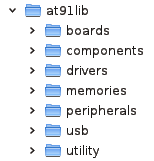
\includegraphics[height=40mm]{../images/ch05/at91lib_dirs.png}
 \caption{Struktura katalogów biblioteki AT91LIB v.1.5}
 \label{fig:AT91LIB}
\end{figure}

Biblioteka AT91LIB jest podzielona na 7 katalogów (rys. \ref{fig:AT91LIB})
odpowiedzialnych za zarządzanie poszczególnymi elementami związanymi z
mikrokontrolerem. W tabeli \ref{tab:AT91LIB} przedstawiono opis funkcjonalności
obsługiwanych przez kod zawarty w poszczególnych katalogach biblioteki. \newpage

\begin{table}[!ht]
\rowcolors{2}{white}{gray!20}
\centering
\caption{Opis poszczególnych katalogów biblioteki AT91LIB v.1.5}
  \begin{tabular}{ | c | c | p{1.75cm} |} \hline
 Nazwa katalogu & Opis \\ \hline
   		boards & obsługa płyt ewaluacyjnych \\
& oraz modułów mikrokontrolerów \\ \hline
   		components & dodatkowe komponenty zewnętrzne \\
& takie jak np. kontroler ethernet \\ \hline
		drivers & wyspecjalizowane wysokopoziomowe \\ 
		 & funkcje zarządzające działaniem \\
& urządzeń peryferyjnych \\ \hline
		memories & obsługa różnego \\ 
& rodzaju pamięci \\ \hline
		peripherals & funkcje niskiego \\
		 & poziomu zarządzające \\ 
& urządzeniami peryferyjnymi \\ \hline usb & obsługa USB \\ \hline
		utility & narzędzia oraz \\ 
& algorytmy dodatkowe \\ \hline
   	\end{tabular}
\label{tab:AT91LIB}
\end{table}

Zastosowanie AT91LIB pozwoliło na stworzenie przejrzystego kodu sterującego
robotem, który będzie można modyfikować bez dokładnego zagłębiania się w notę
katalogową mikrokontrolera AT91SAM7S256.